\documentclass{article}
\PassOptionsToPackage{numbers,compress}{natbib}
\usepackage[preprint]{neurips_2025}

\usepackage[utf8]{inputenc}
\usepackage[T1]{fontenc}
\usepackage[spanish,es-nodecimaldot,es-noquoting]{babel}
\usepackage{hyperref}
\usepackage{url}
\usepackage{booktabs}
\usepackage{amsmath}
\usepackage{amsfonts}
\usepackage{nicefrac}
\usepackage{microtype}
\usepackage{xcolor}
\usepackage{graphicx}
\usepackage{float}
\graphicspath{{fig/}}

\title{Mapeo de inundaciones a partir de radar Sentinel-1 con una U-Net propia: Sen1Floods11 y una región de prueba construida para Lima (2017)}

\author{%
  \textbf{Grupo 6:} Contreras Avendaño, Juan Sebastian Francesco \quad Romero Lovera, Junior \\
  Muñoz Cañabe, Luis \quad Oha Quispe, Derly Raúl \quad Pedraza Palomino, Lourdes \\
  Maestría en Inteligencia Artificial, Facultad de Ingeniería Industrial y de Sistemas \\
  Universidad Nacional de Ingeniería, Lima, Perú \\
  Curso: Redes Neuronales y Aprendizaje Profundo (MIA-203) --- Examen Parcial, Pregunta 2 \\
  Código: \url{https://github.com/loupv99/sen1floods11-unet-lima}
}

\begin{document}
\maketitle

\begin{abstract}
Las nubes que acompañan a las tormentas dejan ciegos a los satélites ópticos justo cuando hay que saber dónde está el agua; el radar de apertura sintética (SAR) de Sentinel-1 las atraviesa. Implementamos desde cero en PyTorch una U-Net que segmenta píxel a píxel el agua de inundación a partir de las bandas VV y VH, y la evaluamos con las particiones oficiales de Sen1Floods11, en la región geográficamente independiente de Bolivia y en una región de prueba que construimos para Lima con la escena Sentinel-1B del 17 de marzo de 2017 y la delineación EMSN038 de Copernicus EMS. En los eventos vistos durante el entrenamiento, la U-Net alcanza un IoU de agua de 0.657 (dos semillas: 0.658 y 0.656) frente a 0.554 de la línea base de Otsu, con 36\,\% menos falsos positivos. En Bolivia la ventaja desaparece (0.657 frente a 0.718 de Otsu): la red mantiene una precisión alta (0.856) pero pierde recall (0.740). En Lima, incluso Otsu cae a un IoU de 0.010; mostramos con datos que gran parte de esa caída se debe a la referencia (extensión máxima de la crecida, cartografiada con imagen óptica días después) y al desierto costero, más que al modelo. Una ablación reducida indica que las conexiones de salto ayudan en distribución (+0.019) pero no en la región nueva.
\end{abstract}

\section{Introducción}
Durante una inundación, la respuesta de emergencia necesita mapas de extensión del agua en horas. Los sensores ópticos fallan bajo nubes; el SAR de banda C de Sentinel-1 ilumina la escena con su propio pulso, de día o de noche, y es la herramienta de facto para el mapeo rápido. La física que lo permite es simple: el agua tranquila se comporta como un espejo y refleja el pulso lejos del sensor, por lo que aparece oscura en las polarizaciones VV y VH, mientras que el suelo, la vegetación y la ciudad devuelven más energía.

El Perú tiene un precedente concreto: con El Niño costero de marzo de 2017 se desbordaron el Rímac y el Chillón, y Copernicus EMS delineó las zonas inundadas de Lima en la activación EMSN038 \cite{emsn038}. Este trabajo responde a una pregunta práctica: \emph{¿puede una U-Net entrenada desde cero con Sentinel-1 segmentar el agua de inundación y seguir funcionando en Lima, una región que nunca vio?} Nuestras contribuciones son: (i) una U-Net propia en PyTorch con entrada VV/VH (E1); (ii) una ablación de la arquitectura de saltos (E2); (iii) una evaluación en distribución con IoU, F1, precisión, recall y matrices de confusión comentadas (E3); (iv) una región de prueba de Lima construida con dos fuentes independientes y la medición de la brecha de generalización con hipótesis contrastadas (E4); y (v) un análisis de los fallos característicos del SAR (E5).

\section{Trabajos relacionados}
La U-Net \cite{ronneberger2015} introdujo la arquitectura codificador--decodificador con conexiones de salto por concatenación para segmentación densa con pocos datos; variantes como Attention U-Net \cite{oktay2018} y UNet++ \cite{zhou2018} refinan el diseño de los saltos. Para el agua superficial, Isikdogan et~al.~\cite{isikdogan2017} mostraron que las redes convolucionales superan a los índices espectrales clásicos. Sen1Floods11 \cite{bonafilia2020} es el conjunto de referencia para inundaciones con Sentinel-1: 11 eventos, 446 chips etiquetados a mano y 4\,384 chips con etiquetas débiles; sus autores reportan que entrenar con etiquetas débiles puede igualar o superar al entrenamiento con pocas etiquetas expertas. Los métodos de umbral, en particular Otsu \cite{otsu1979}, siguen siendo la línea base operativa del mapeo SAR. Las inundaciones urbanas son un caso difícil porque el agua y las paredes forman un reflector de doble rebote que brilla en lugar de oscurecerse \cite{mason2014}; la coherencia interferométrica se ha propuesto para detectarlas \cite{chini2019}. La pérdida Dice \cite{milletari2016} es la opción habitual ante el fuerte desbalance de clases de la segmentación de agua, y la capa JRC de agua superficial \cite{pekel2016} sirve para separar el agua permanente.

\section{Datos}
\subsection{Sen1Floods11}
Usamos la versión 1.1 del bucket público del conjunto \cite{bonafilia2020}. Cada chip mide $512\times512$ píxeles de unos 10\,m ($8.98315\times10^{-5}$ grados en EPSG:4326, medido en los archivos) y trae dos bandas SAR en dB (VV, VH). La Tabla~\ref{tab:datos} resume lo que medimos. Dos hechos condicionan todo el trabajo: el agua es una clase muy minoritaria (9.5\,\% de los píxeles válidos del entrenamiento), y las etiquetas débiles derivadas de Sentinel-1 son un umbral de Otsu sobre la propia imagen, que coincide solo 0.45 (IoU) con la etiqueta dorada; por evento, va de 0.78 (Mekong) a 0.15 (Pakistán y Somalia), donde el terreno árido oscuro se confunde con agua.

\begin{table}[H]
\centering
\caption{Hechos del conjunto medidos sobre los archivos (no tomados del enunciado).}
\label{tab:datos}
\small
\begin{tabular}{lr}
\toprule
Chips dorados (entrenamiento / validación / test / Bolivia) & 446 (252 / 89 / 90 / 15) \\
Chips débiles (los mismos chips con dos etiquetas: Otsu-S1 y S2) & 4\,384 \\
Fracción de agua en píxeles válidos (train / test / Bolivia) & 9.5\,\% / 12.5\,\% / 15.9\,\% \\
Píxeles sin dato (NaN) en las imágenes S1 & 2.15\,\% \\
IoU de la etiqueta débil Otsu-S1 frente a la dorada (train) & 0.45 \\
\bottomrule
\end{tabular}
\end{table}

\subsection{Región de prueba de Lima}
Sen1Floods11 no incluye eventos peruanos, así que construimos una región con dos fuentes independientes (Figura~\ref{fig:lima}).
\textbf{Imagen.} Buscamos en el catálogo las escenas Sentinel-1 sobre Lima en marzo de 2017; la más cercana a la delineación óptica es la de Sentinel-1B del 17 de marzo de 2017, 10:38 UTC, pasada descendente, órbita relativa 171, VV+VH. La obtuvimos como producto RTC ($\gamma^0$ con terreno aplanado) del Microsoft Planetary Computer \cite{planetary}, la reproyectamos a EPSG:4326 con la grilla de Sen1Floods11 y la convertimos a $\sigma^0$ en dB con
$\sigma^0_{\mathrm{dB}}=\gamma^0_{\mathrm{dB}}+10\log_{10}\cos\theta$, donde $\theta$ es el ángulo de incidencia interpolado de la anotación del producto (43.3--46.4$^\circ$ en Lima; corrección media de $-1.51$\,dB). Como control, las medias de la escena (VV $-9.95$, VH $-17.24$\,dB) coinciden con las del entrenamiento de Sen1Floods11 (VV $-10.40$, VH $-17.24$\,dB).
\textbf{Etiquetas.} Descargamos la geodatabase oficial de EMSN038 \cite{emsn038} y usamos la capa \texttt{Potential\_Maximum\_flood} (13 polígonos, 13.58\,km$^2$), rasterizada en la misma grilla. Solo rotulamos el área de interés intersectada con las huellas de las imágenes WorldView-2 del 18 y 21 de marzo; fuera de ella no hay delineación y el píxel se ignora. Resultado: 51 chips de $512\times512$, con 1.25\,\% de píxeles válidos inundados.
\textbf{Límite (parte de la evaluación).} Esta referencia no es verdad de terreno: proviene de imagen óptica de mayor resolución, de 1 a 4 días después del pase del radar, y marca la extensión \emph{máxima} de la crecida en un producto de \emph{Risk \& Recovery}, que incluye lodo y depósitos de huaico, no necesariamente agua abierta el 17 de marzo.

\begin{figure}[H]
\centering
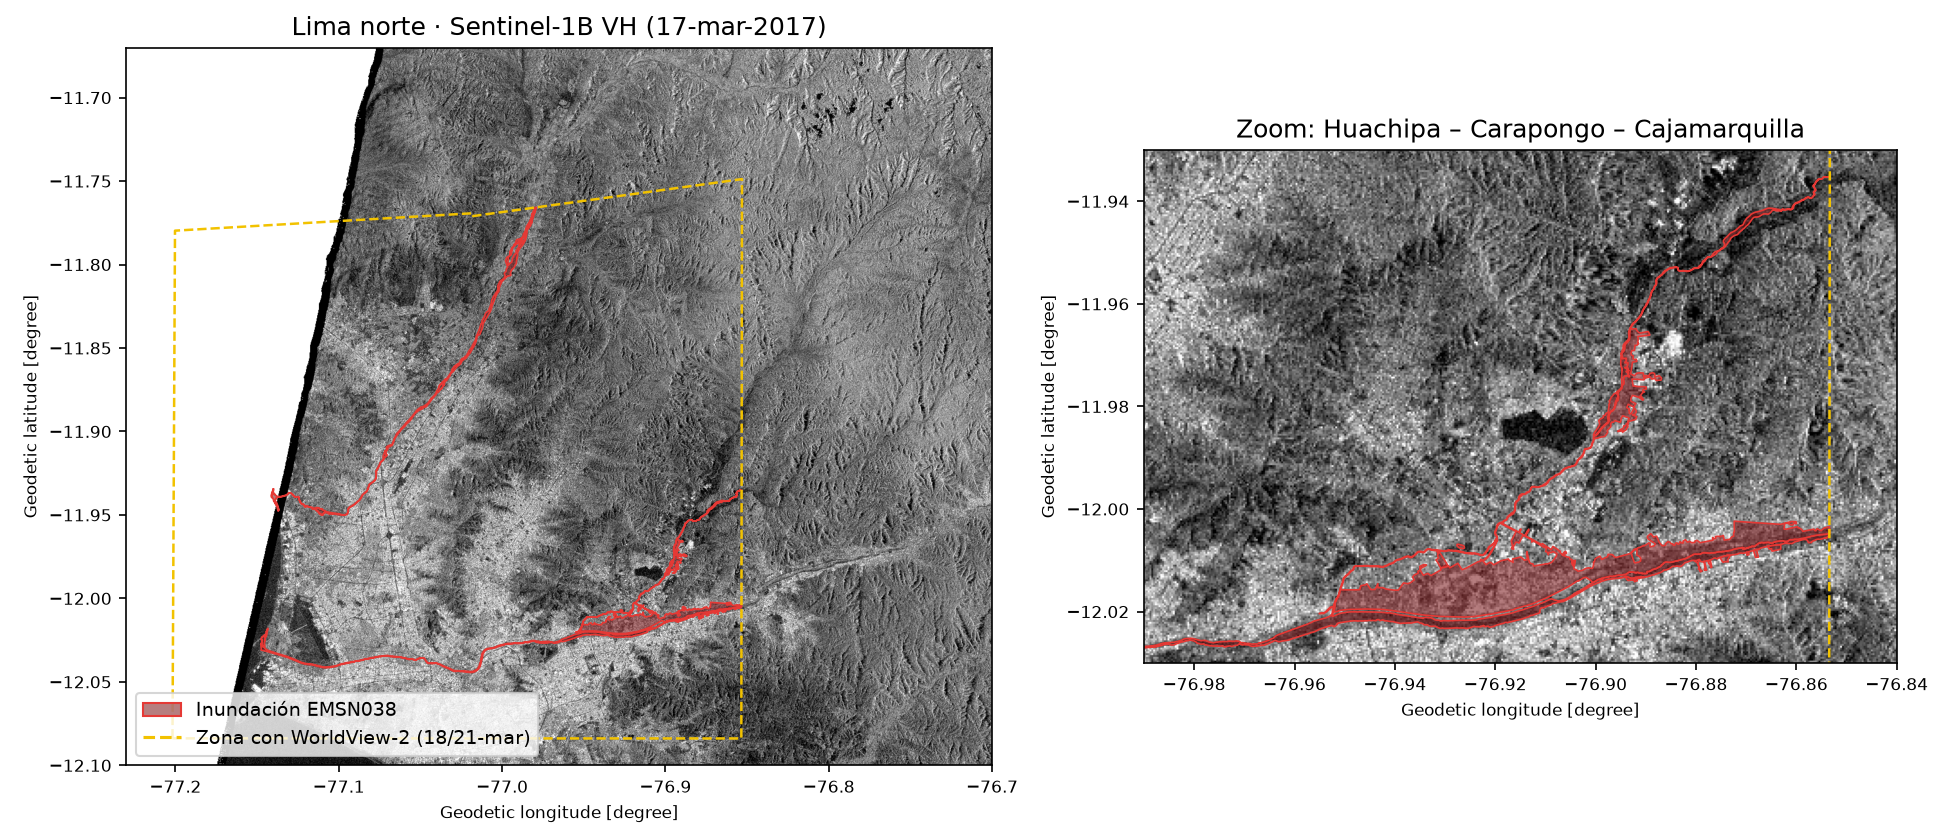
\includegraphics[width=\linewidth]{06_lima_mapa.png}
\caption{Región de prueba de Lima: Sentinel-1B VH del 17-mar-2017 con los polígonos de inundación de EMSN038 (rojo) y la zona cubierta por WorldView-2 (amarillo). En Huachipa y Carapongo, dentro de los polígonos, el radar no se ve oscuro como el agua abierta.}
\label{fig:lima}
\end{figure}

\section{Método}
\textbf{Arquitectura (E1).} La U-Net recibe 2 canales (VV, VH). Cada bloque aplica dos veces convolución $3\times3$ con relleno 1, BatchNorm y ReLU; el codificador tiene 5 niveles (32, 64, 128, 256 y 512 canales, de $512^2$ a $32^2$) unidos por max-pooling $2\times2$, y el decodificador sube con convoluciones transpuestas $2\times2$ y concatena el mapa del nivel correspondiente del codificador. Una convolución $1\times1$ produce un logit por píxel. El modelo tiene 7\,762\,753 parámetros (el conteo a mano coincide con PyTorch) y usa solo \texttt{torch.nn}, sin bibliotecas de segmentación. Las variantes de la ablación eliminan los saltos o reducen la base de canales.
\textbf{Preprocesamiento.} Los NaN se marcan como píxeles no válidos (etiqueta $-1$, sin gradiente); los valores se recortan a $[-50,1]$\,dB y se estandarizan con la media y la desviación del entrenamiento dorado. Como aumento usamos solo volteos: no rotamos, porque el radar mira de lado y la sombra cae siempre hacia el mismo lado.
\textbf{Pérdida.} Por el desbalance (9.5\,\% de agua) combinamos BCE con \texttt{pos\_weight} $=9.52$ (cociente no-agua/agua medido) y Dice suave calculada sobre el lote, ambas sobre píxeles válidos.
\textbf{Métricas.} Para la clase agua: $\mathrm{IoU}=\frac{TP}{TP+FP+FN}$, F1, precisión y recall, agregados sumando los píxeles de todos los chips; omisión $=1-$recall y comisión $=1-$precisión. Reportamos también la media de IoU por chip (excluyendo chips sin agua), que es la métrica de los autores del conjunto.
\textbf{Protocolo.} La época y el umbral de decisión se eligen en validación; test, Bolivia y Lima nunca intervienen en una decisión. Los chips débiles de Bolivia se excluyen para que sea una región no vista. La línea base es Otsu sobre VH, con un umbral por escena.

\section{Experimentos y resultados}
\textbf{Configuración.} El modelo completo (\texttt{A\_dorado}) se entrenó en Google Colab con GPU T4 sobre los 252 chips dorados: 60 épocas, AdamW (lr $5\times10^{-4}$, decaimiento $10^{-2}$), OneCycle, lotes de 16 y recortes de $256\times256$; cada corrida tarda unos 2.9 minutos. Reportamos dos semillas. La ablación de saltos se corrió en CPU con una U-Net reducida (base 16, 1.94 M parámetros, 20 épocas, lotes de 8, una semilla), por lo que sus cifras son indicativas.

\subsection{Evaluación en distribución (E3)}
En los 90 chips de test, de los mismos eventos vistos en entrenamiento, la U-Net supera a Otsu en todas las métricas (Tabla~\ref{tab:res}, Figura~\ref{fig:iou}): IoU 0.657 frente a 0.554 (+0.10), con precisión 0.796 frente a 0.682 y recall 0.790 frente a 0.748. Las dos semillas difieren en 0.0014 de IoU, de modo que la mejora no es ruido de inicialización. Por evento (corrida reducida), la U-Net gana en Paraguay (0.56 frente a 0.38), Somalia (0.47 frente a 0.37), Mekong (0.85 frente a 0.75) y España (0.70 frente a 0.62), y empata en India (0.70) y Pakistán (0.19 frente a 0.18), donde el terreno árido es difícil para ambos.

\begin{table}[H]
\centering
\caption{Resultados de la clase agua. U-Net: media de las semillas 0 y 1 (Colab T4). mIoU/chip: media por chip, excluyendo chips sin agua.}
\label{tab:res}
\small
\begin{tabular}{llcccccc}
\toprule
Región & Método & IoU & F1 & Precisión & Recall & Omisión & Comisión \\
\midrule
Test & U-Net & \textbf{0.657} & \textbf{0.793} & \textbf{0.796} & \textbf{0.790} & 0.210 & 0.204 \\
     & Otsu-VH & 0.554 & 0.713 & 0.682 & 0.748 & 0.252 & 0.318 \\
\midrule
Bolivia & U-Net & 0.657 & 0.793 & \textbf{0.856} & 0.740 & 0.260 & 0.144 \\
        & Otsu-VH & \textbf{0.718} & \textbf{0.836} & 0.803 & \textbf{0.870} & 0.130 & 0.197 \\
\midrule
Lima & Otsu-VH & 0.010 & 0.021 & 0.011 & 0.442 & 0.558 & 0.989 \\
\bottomrule
\end{tabular}

\vspace{2pt}
\begin{tabular}{lccc}
\toprule
mIoU/chip & Validación & Test & Bolivia \\
\midrule
U-Net (semillas 0 / 1) & 0.378 / 0.385 & 0.385 / 0.397 & 0.390 / 0.413 \\
Otsu-VH & 0.319 & 0.332 & 0.474 \\
\bottomrule
\end{tabular}
\end{table}

\begin{figure}[H]
\centering
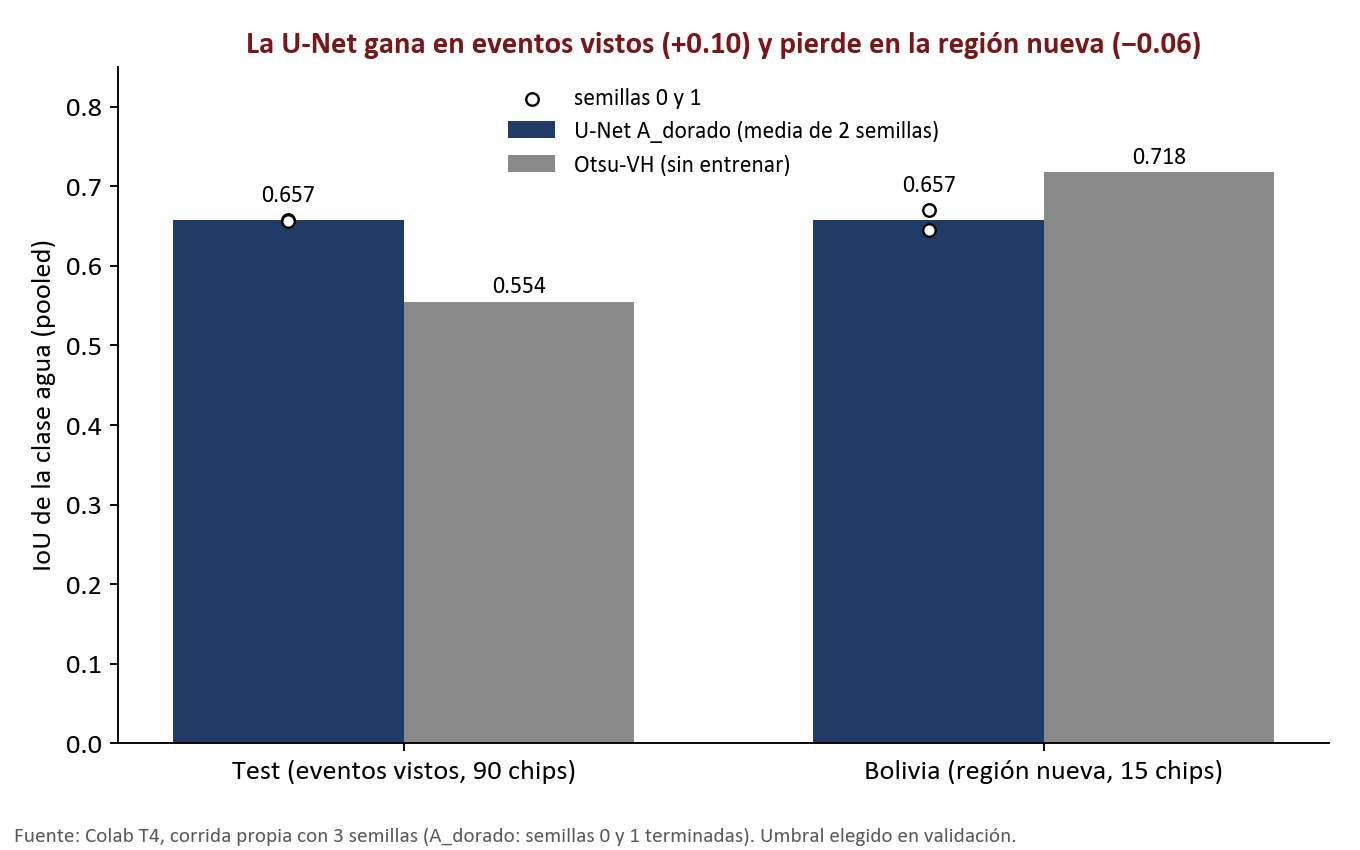
\includegraphics[width=0.62\linewidth]{01_iou_unet_vs_otsu.png}
\caption{IoU de agua en test y en Bolivia. Barras: media; puntos: cada semilla.}
\label{fig:iou}
\end{figure}

\textbf{Matriz de confusión comentada.} La Figura~\ref{fig:cm} muestra las matrices en píxeles. (i) La exactitud engaña: el 87.7\,\% de los píxeles de test es no-agua, así que Otsu logra 92.6\,\% de exactitud con un IoU de solo 0.55. (ii) La U-Net reduce los falsos positivos un 36\,\% (876\,827 $\to$ 559\,258): no toma toda superficie oscura por agua porque usa el contexto espacial. (iii) También reduce los falsos negativos un 17\,\% (634\,364 $\to$ 526\,718). (iv) En Lima, Otsu marca como agua el 52\,\% de la zona.

\begin{figure}[H]
\centering
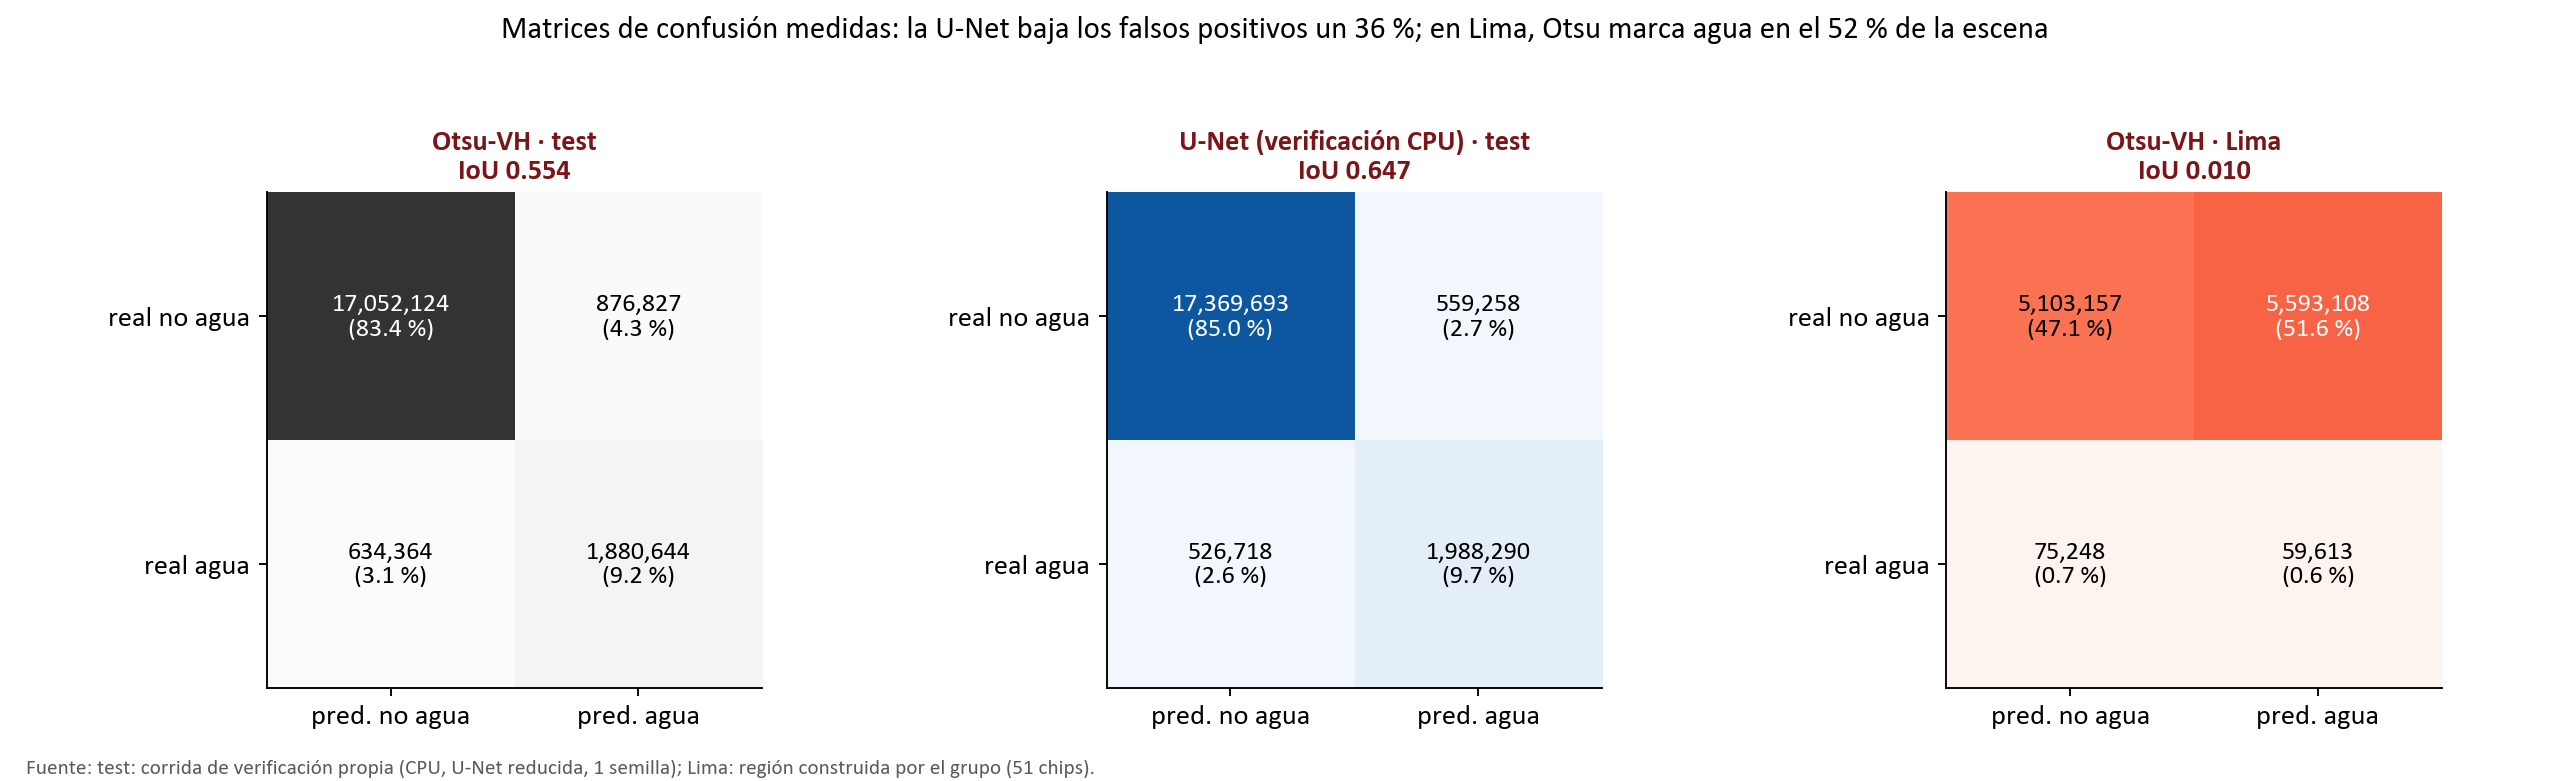
\includegraphics[width=\linewidth]{03_matrices_confusion.png}
\caption{Matrices de confusión medidas. Izquierda: Otsu en test. Centro: U-Net reducida en test (corrida de verificación, una semilla). Derecha: Otsu en Lima.}
\label{fig:cm}
\end{figure}

\subsection{Ablación de arquitectura (E2)}
Al quitar las conexiones de salto (Figura~\ref{fig:saltos}), el IoU en test baja de 0.647 a 0.628: los saltos devuelven al decodificador los bordes y cauces delgados que se pierden al reducir la resolución a $32\times32$. En Bolivia ocurre lo contrario (0.578 con saltos frente a 0.624 sin ellos): el detalle fino aprendido en los eventos de entrenamiento no se transfiere a una escena nueva. Además, pasar del modelo reducido (1.94 M parámetros) al completo (7.76 M) sube el IoU en test de 0.647 a 0.657.

\begin{figure}[H]
\centering
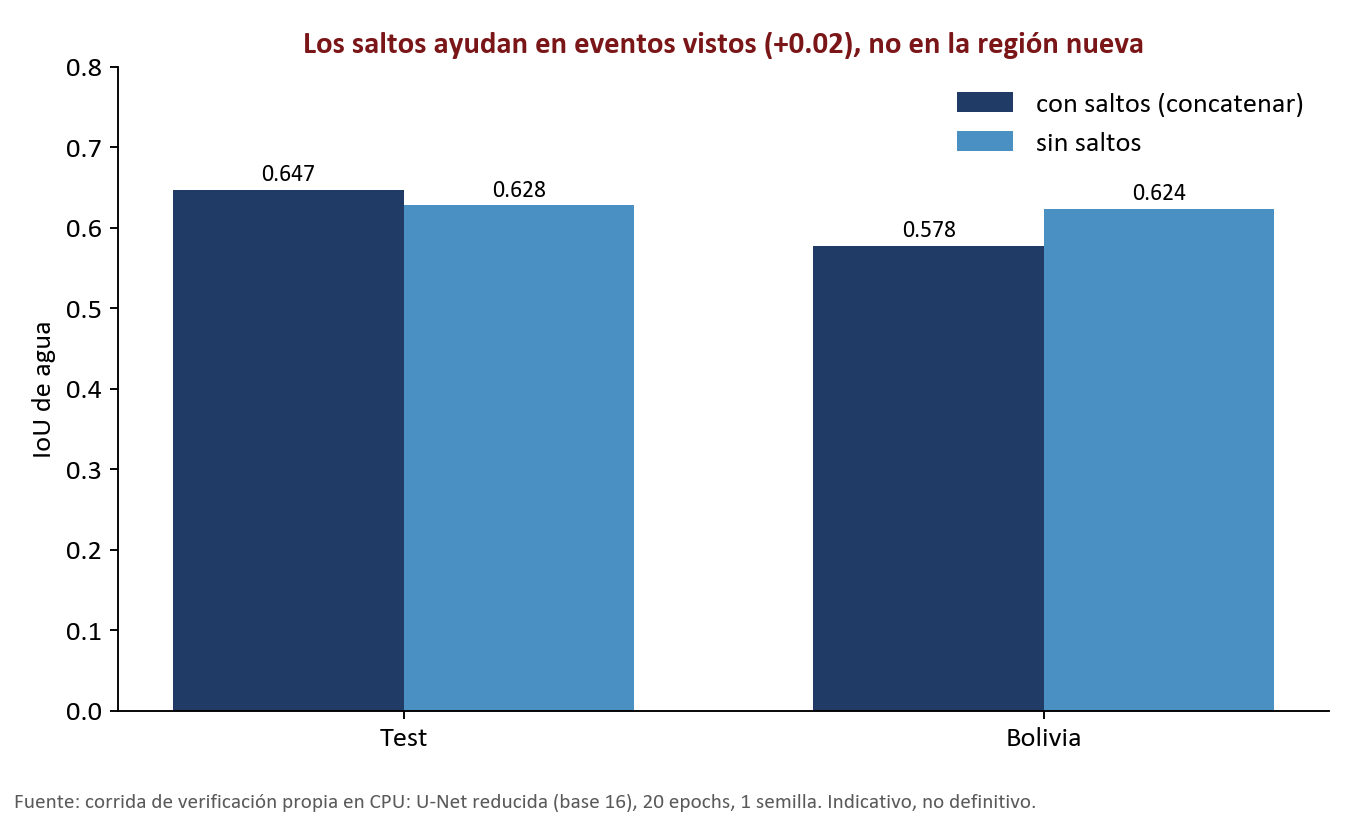
\includegraphics[width=0.55\linewidth]{05_saltos_cpu.png}
\caption{Ablación de las conexiones de salto (U-Net reducida, una semilla).}
\label{fig:saltos}
\end{figure}

\subsection{Generalización geográfica (E4)}
\textbf{Bolivia.} El IoU de la U-Net se mantiene (0.657), pero Otsu sube de 0.554 a 0.718, de modo que la ventaja del modelo desaparece (Figura~\ref{fig:bol}). La red sigue siendo precisa (0.856) pero se le escapa agua (recall 0.740 frente a 0.870). Otsu recalcula su umbral en cada escena, mientras que la red aplica una función y un umbral fijos aprendidos en otros eventos.

\begin{figure}[H]
\centering
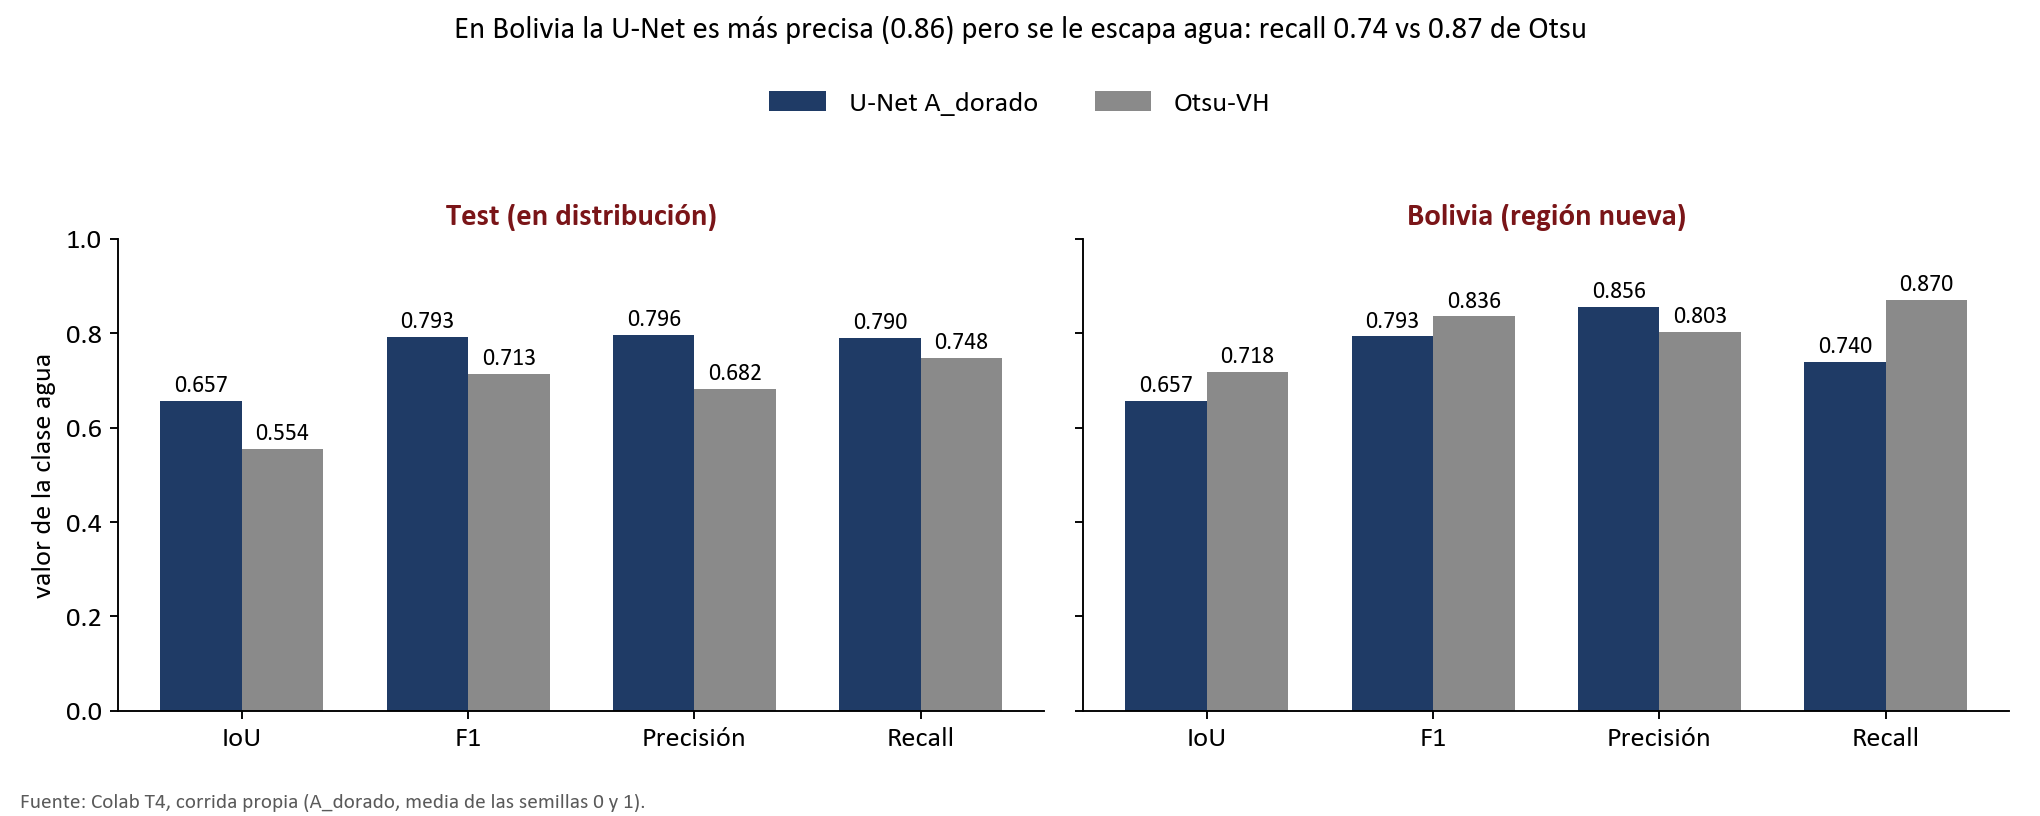
\includegraphics[width=0.9\linewidth]{02_metricas_test_bolivia.png}
\caption{IoU, F1, precisión y recall en test y en Bolivia.}
\label{fig:bol}
\end{figure}

\textbf{Lima.} En la región construida, la línea base de Otsu cae a un IoU de 0.010 (Figura~\ref{fig:limaotsu}): la brecha frente al test es de 0.54 sin que intervenga ningún modelo aprendido. El umbral de Otsu de la escena es $-16.9$\,dB, frente a $-20$ a $-25$\,dB en los eventos de Sen1Floods11: en Lima el histograma separa desierto de ciudad, no agua de tierra. Proponemos y contrastamos cinco hipótesis sobre la brecha:
\textbf{H1, desajuste temporal y de fenómeno:} la referencia marca la extensión máxima (lodo, sedimentos) de 1 a 4 días después; en la Figura~\ref{fig:lima} el radar no ve agua abierta dentro de los polígonos.
\textbf{H2, desierto costero:} la arena seca y lisa es oscura como el agua y desplaza el umbral.
\textbf{H3, escala extrema:} solo 1.25\,\% de los píxeles son agua, así que pocos falsos positivos hunden el IoU.
\textbf{H4, geometría del radar:} Lima queda en el extremo lejano de la pasada (43--46$^\circ$, órbita descendente), con laderas que producen sombra.
\textbf{H5, doble rebote urbano:} el agua entre edificios brilla \cite{mason2014}, y Sen1Floods11 no contiene inundaciones urbanas \cite{bonafilia2020}.
H1--H4 están respaldadas por las mediciones anteriores; H5 no puede verificarse con estos datos.

\begin{figure}[H]
\centering
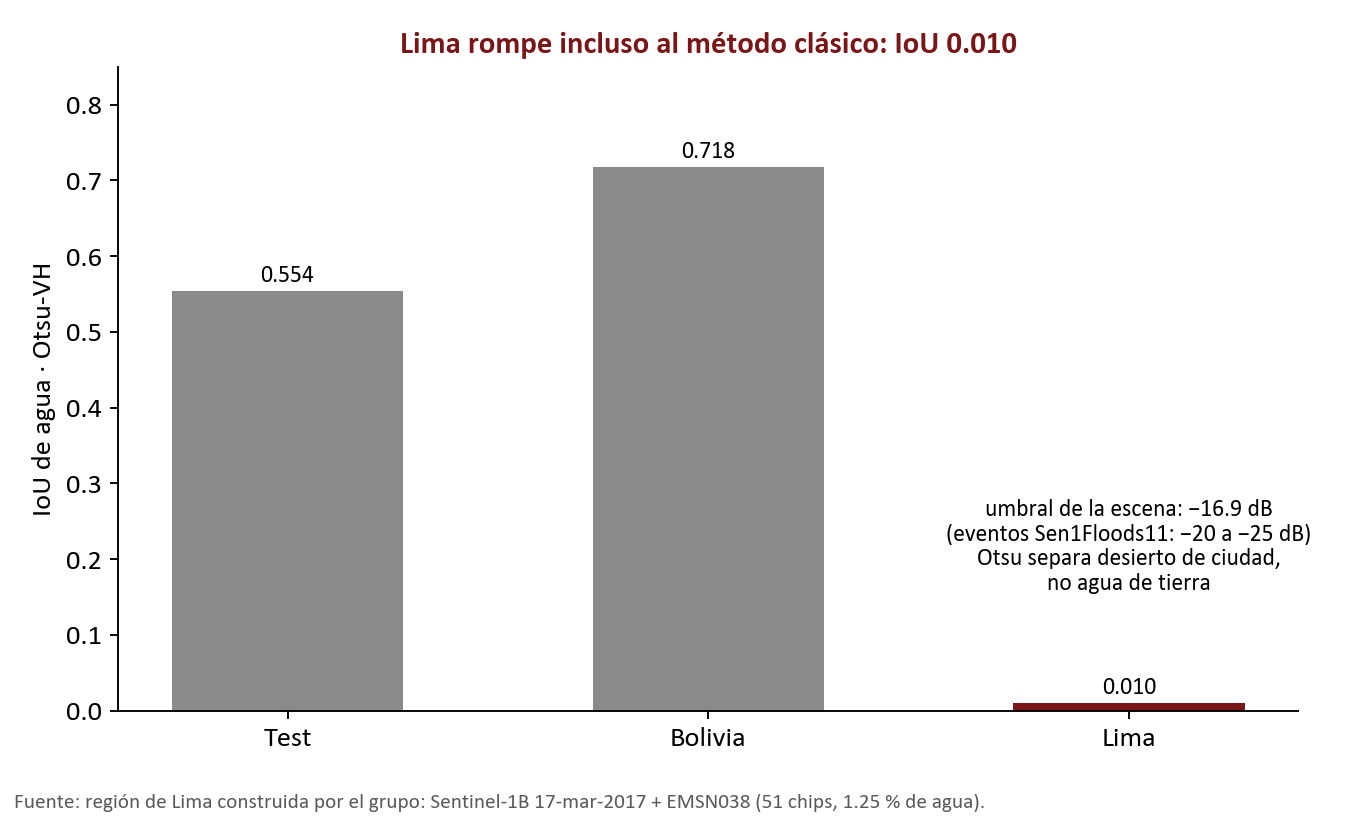
\includegraphics[width=0.55\linewidth]{04_lima_otsu.png}
\caption{IoU de Otsu-VH en test, Bolivia y Lima.}
\label{fig:limaotsu}
\end{figure}

\subsection{Fallos característicos del SAR (E5)}
Clasificamos los errores de la U-Net en test con umbrales físicos simples y revisamos los ejemplos. (1) \textbf{Superficies oscuras que no son agua} (arena, asfalto, suelo húmedo y liso): el 60\,\% de los falsos positivos tiene VH $<-22$\,dB. (2) \textbf{Agua brillante} (vegetación inundada, doble rebote): el 67\,\% de los falsos negativos tiene VV $>-12$\,dB, es decir, agua que el radar no ve como espejo; incluye casos donde la etiqueta, dibujada sobre la imagen óptica, marca agua que el SAR no registra. (3) \textbf{Bordes}: el 51\,\% de los falsos negativos está en el contorno, donde un píxel de 10\,m es mitad agua y mitad tierra. (4) \textbf{Speckle}: el 14\,\% de los falsos positivos son manchas aisladas de menos de 20 píxeles. La \textbf{sombra de radar} en laderas actúa como el tipo (1) y es la explicación más probable de los falsos positivos en los cerros de Lima (H4).

\section{Discusión y limitaciones}
La U-Net aprende algo que el umbral no captura dentro de la distribución, pero la ventaja no se transfiere sola: en una región nueva, un método que se recalibra en cada escena compite mejor. Esto sugiere normalizar cada escena con sus propias estadísticas o recalibrar el umbral en la región de destino antes de desplegar el modelo. En Lima, que Otsu también fracase muestra que la brecha mezcla error del modelo con desacuerdo de la referencia; por eso un IoU bajo en Lima no debe leerse solo como falla de la red.
Limitaciones: dos semillas para el modelo completo y una para la ablación reducida; Bolivia tiene solo 15 chips; la referencia de Lima no es verdad de terreno en la fecha del radar, y la conversión de $\gamma^0$ a $\sigma^0$ es exacta en terreno llano pero aproximada en laderas. La comparación entre entrenar solo con etiquetas doradas y añadir las débiles no se completó en el plazo de esta entrega.

\section{Conclusión}
Una U-Net propia con VV y VH supera a la línea base de Otsu en los eventos conocidos de Sen1Floods11 (IoU 0.657 frente a 0.554), de forma estable entre semillas y con 36\,\% menos falsos positivos. Fuera de la distribución, la ventaja desaparece en Bolivia y, en la región de Lima que construimos, incluso el método clásico se rompe (IoU 0.010) por una combinación de referencia óptica de extensión máxima, desierto costero y escala extrema. El código, el cuaderno de Colab y la construcción de Lima son reproducibles con un solo comando en \url{https://github.com/loupv99/sen1floods11-unet-lima}.

\begin{thebibliography}{12}
\bibitem{bonafilia2020} D.~Bonafilia, B.~Tellman, T.~Anderson y E.~Issenberg. Sen1Floods11: a georeferenced dataset to train and test deep learning flood algorithms for Sentinel-1. En \emph{CVPR Workshops}, pp.~210--211, 2020.
\bibitem{chini2019} M.~Chini, R.~Pelich, L.~Pulvirenti, N.~Pierdicca, R.~Hostache y P.~Matgen. Sentinel-1 InSAR coherence to detect floodwater in urban areas: Houston and Hurricane Harvey as a test case. \emph{Remote Sensing}, 11(2):107, 2019.
\bibitem{emsn038} Copernicus Emergency Management Service. EMSN038: Post-disaster situation analyses of flood and landslides in Lima, Peru. \url{https://mapping.emergency.copernicus.eu/activations/EMSN038/}. Consultado el 31-oct-2026.
\bibitem{isikdogan2017} F.~Isikdogan, A.~C.~Bovik y P.~Passalacqua. Surface water mapping by deep learning. \emph{IEEE J. Sel. Top. Appl. Earth Obs. Remote Sens.}, 10(11):4909--4918, 2017.
\bibitem{mason2014} D.~C.~Mason, L.~Giustarini, J.~Garcia-Pintado y H.~L.~Cloke. Detection of flooded urban areas in high resolution synthetic aperture radar images using double scattering. \emph{Int. J. Appl. Earth Obs. Geoinf.}, 28:150--159, 2014.
\bibitem{milletari2016} F.~Milletari, N.~Navab y S.-A.~Ahmadi. V-Net: fully convolutional neural networks for volumetric medical image segmentation. En \emph{3DV}, pp.~565--571, 2016.
\bibitem{oktay2018} O.~Oktay et~al. Attention U-Net: learning where to look for the pancreas. En \emph{MIDL}, 2018.
\bibitem{otsu1979} N.~Otsu. A threshold selection method from gray-level histograms. \emph{IEEE Trans. Syst., Man, Cybern.}, 9(1):62--66, 1979.
\bibitem{pekel2016} J.-F.~Pekel, A.~Cottam, N.~Gorelick y A.~S.~Belward. High-resolution mapping of global surface water and its long-term changes. \emph{Nature}, 540:418--422, 2016.
\bibitem{planetary} Microsoft Planetary Computer. Sentinel-1 Radiometrically Terrain Corrected (RTC). \url{https://planetarycomputer.microsoft.com/dataset/sentinel-1-rtc}. Consultado el 31-oct-2026.
\bibitem{ronneberger2015} O.~Ronneberger, P.~Fischer y T.~Brox. U-Net: convolutional networks for biomedical image segmentation. En \emph{MICCAI}, pp.~234--241, 2015.
\bibitem{zhou2018} Z.~Zhou, M.~M.~R.~Siddiquee, N.~Tajbakhsh y J.~Liang. UNet++: a nested U-Net architecture for medical image segmentation. En \emph{DLMIA}, pp.~3--11, 2018.
\end{thebibliography}

\end{document}
